\documentclass[12pt]{article}
\usepackage{graphicx}
\usepackage{rotating}
\pagestyle{empty}
\usepackage{ragged2e}
\usepackage{authblk}
\usepackage{geometry}
\newgeometry{scale=.9}
\usepackage[urlcolor=blue,citecolor=black,linkcolor=black,colorlinks=True,breaklinks=True]{hyperref}
\usepackage{caption}
\captionsetup[figure]{labelfont={bf},name={Figure},labelsep=period}
\captionsetup[table]{labelfont={bf},name={Table},labelsep=period}
\renewcommand*{\thefigure}{S\arabic{figure}}
\renewcommand*{\thetable}{S\arabic{table}}
\usepackage{multirow}
\usepackage{booktabs}
\usepackage{float}
\usepackage{threeparttable}
\usepackage{caption}

\title{Supporting Information for\\ \textbf{Deep learning and transfer learning of earthquake and quarry-blast discrimination: Applications to southern
California and eastern Kentucky}}
\author[1]{Jun Zhu}
\author[2]{Lihua Fang}
\author[3]{Fajun Miao}
\author[2]{Liping Fan}
\author[1]{Ji Zhang}
\author[1,4]{Zefeng Li\thanks{Corresponding author: zefengli@mail.ustc.edu.cn}}
\affil[1]{Laboratory of Seismology and Physics of Earth’s Interior, School of Earth and Space Science, University of Science and Technology of China, 230026, Hefei, China.}
\affil[2]{Institute of Geophysics, China Earthquake Administration, 100081, Beijing, China.}
\affil[3]{Jiangsu Earthquake Administration, China Earthquake Administration, 210014, Nanjing, China.}
\affil[4]{Mengcheng National Geophysical Observatory, University of Science and Technology of China, 233500, Mengcheng, China.}
\renewcommand*{\Affilfont}{\small\it}
\renewcommand*{\Authfont}{\bf}
\renewcommand\Authands{ and }
\date{*Corresponding author: Zefeng Li (\href{mailto:zefengli@ustc.edu.cn}{zefengli@ustc.edu.cn})\\\it{Manuscript submitted to Geophysical Journal International\\ \today}}

\begin{document}
\begin{titlepage}
\newgeometry{scale=.75}
\maketitle
\setcounter{page}{0}
\thispagestyle{empty}
\end{titlepage}

\begin{figure}
	\centering
	\includegraphics[width=.8\textwidth]{station_cal.pdf}
	\caption{Seismic stations in the California data set, coloured by different networks.}
        \label{station_cal}
\end{figure}

\begin{figure}
        \centering
	\includegraphics[width=.9\textwidth]{hist_socal_side_bar.pdf}
	\caption{Histograms of (a) magnitude, (b) depth, (c) epicentral distance and (d) SNR of the California data set.}
\end{figure}

\begin{figure}
	\centering
	\includegraphics[width=.8\textwidth]{station_ek.pdf}
	\caption{Seismic stations in the Kentucky data set. Note that EKMMP,
abbreviated as EK, is a part of the temporary Eastern Kentucky Microseismic Monitoring Network.}
        \label{station_ek}
\end{figure}

\begin{figure}
        \centering
	\includegraphics[width=.9\textwidth]{hist_ek_side_bar.pdf}
	\caption{Histograms of (a) magnitude, (b) depth, (c) epicentral distance and (d) SNR of the Kentucky data set. The magnitude and depth of the blasts are not available.}
\end{figure}

\begin{figure}
        \centering
	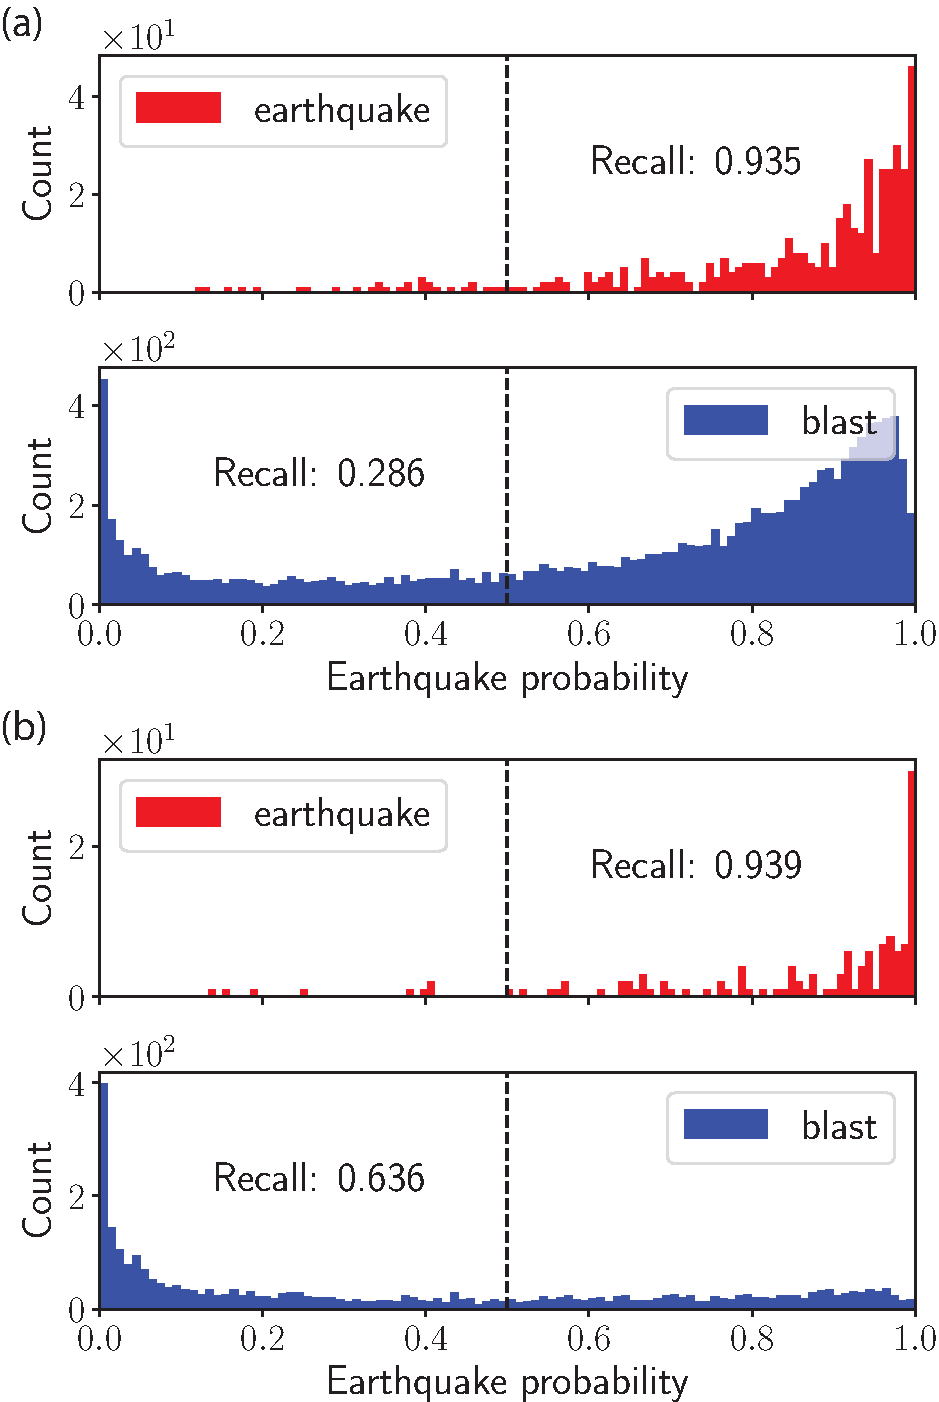
\includegraphics[width=.5\textwidth]{socal_ek.pdf}
	\caption{The performances of the original California model on the Kentucky test set. (a) Histograms of the earthquake probabilities, predicted by the California model, for the entire Kentucky test set. (b) Same as (a) but the samples with \textgreater{100}-km epicentral distances have been removed.}
\end{figure}

\begin{figure}
        \centering
	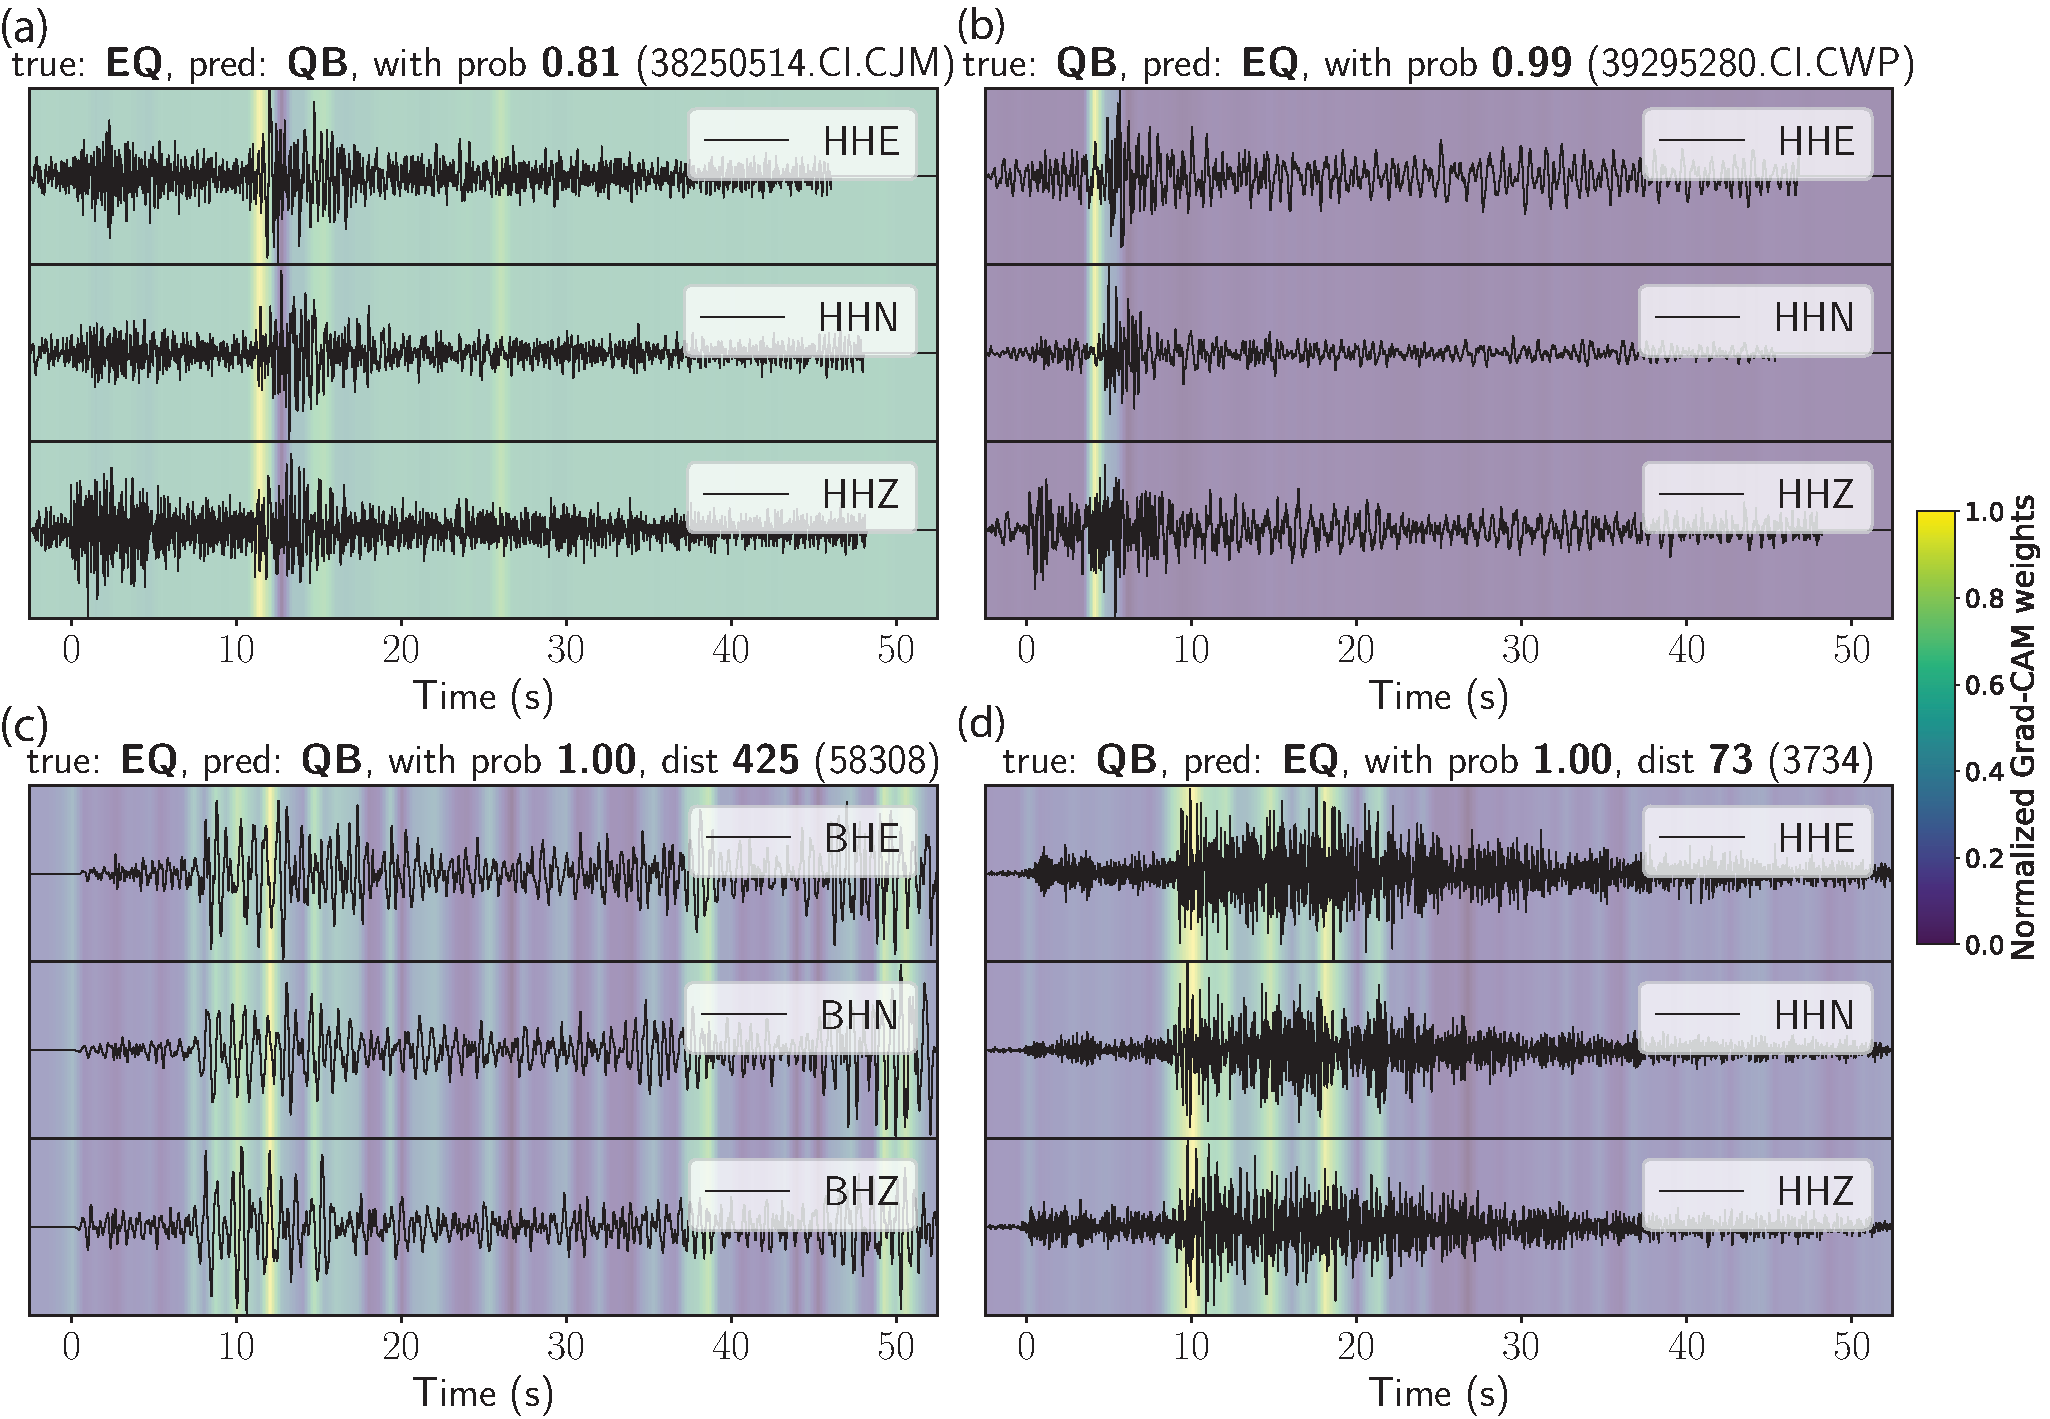
\includegraphics[width=.98\textwidth]{grad_CAM_misprediction.pdf}
	\caption{Grad-CAM tests for four mispredictions in (a-b) southern California and (c-d) eastern Kentucky. Symbols are similar to those in Figs.~8 and 9.}
\end{figure}

\begin{figure}
	\centering
	\includegraphics[width=.5\textwidth]{tradeoff.pdf}
	\caption{Trade-off between model complexity and accuracy.}
\end{figure}

\begin{figure}
	\centering
	\includegraphics[width=.98\textwidth]{false_positive.pdf}
	\caption{Distribution of false positives and potential mislabels in the California test set. The red and the blue dots are earthquakes and blasts labelled by SCSN analysts. The circles and the star mark 20 false positives colour-coded by event depth, among which 7 are potential mislabels annotated by corresponding SCEDC event IDs and listed in Table~\ref{mislabel}.}
        \label{false_blast}
\end{figure}

\begin{figure}
	\centering
	\includegraphics[width=.98\textwidth]{false_negative.pdf}
	\caption{Distribution of false negatives and potential mislabels in the California test set. Symbols are similar to those in Fig.~\ref{false_blast}.}
\end{figure}

\begin{figure}
	\centering
	\includegraphics[width=.5\textwidth]{hist_nstation.pdf}
	\caption{Probability density functions of the number of available stations for the test events in Kentucky (blue) and California (orange)). Each test event has 13 stations on average in Kentucky and 21 in California.}
\end{figure}

\begin{figure}
        \centering
	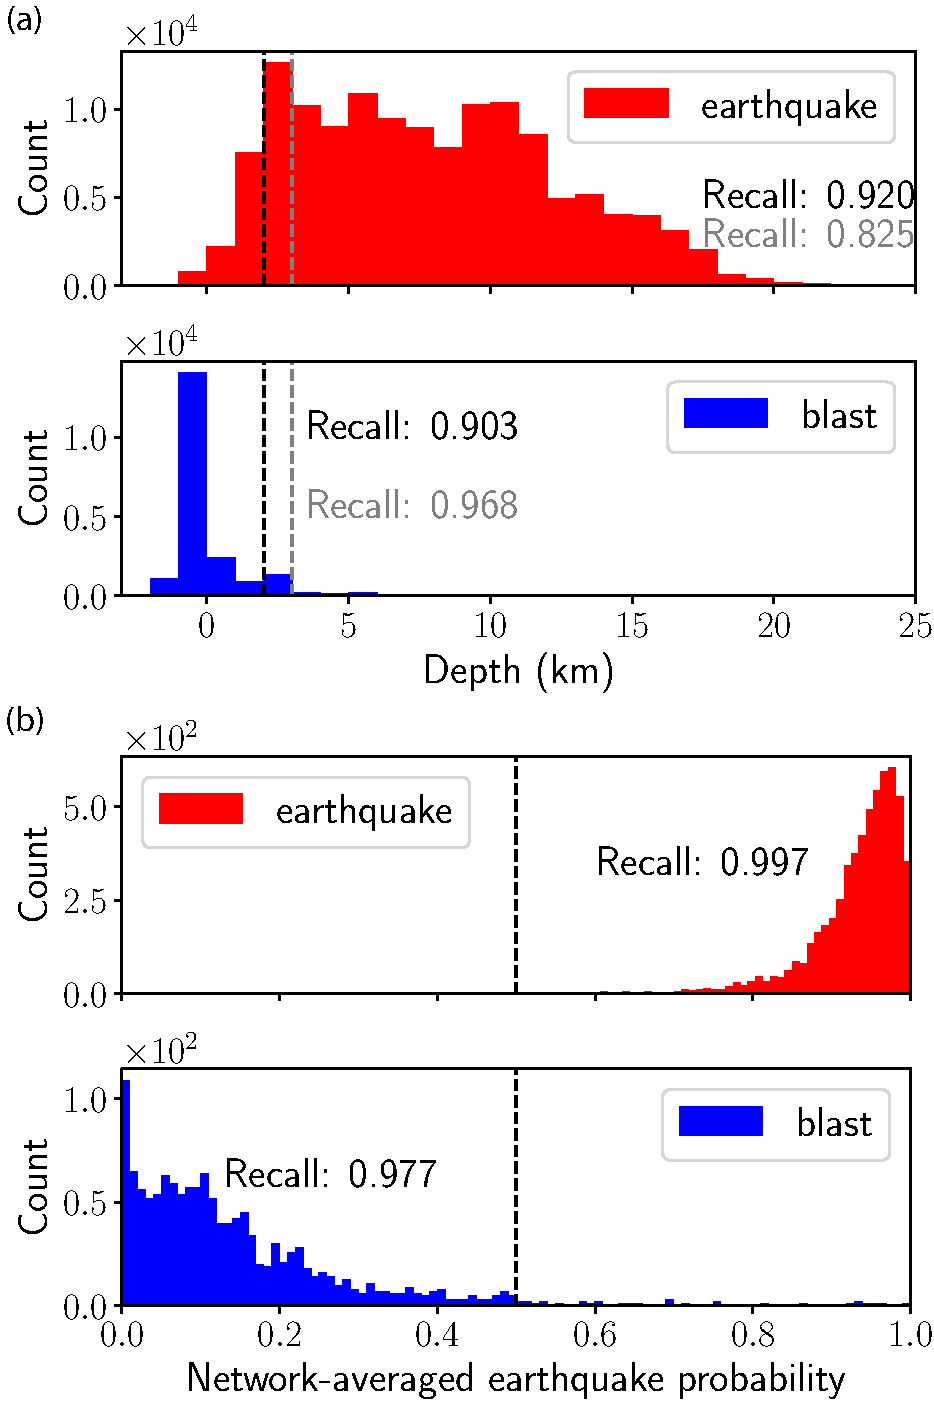
\includegraphics[width=.5\textwidth]{depth_vs_networkaverage.pdf}
	\caption{Event classification according to (a) depth and (b) network-averaged earthquake probability for the California test set. (a) With 2 km as the depth threshold (black dashed line), the recalls for earthquakes and blasts are 92.0\% and 90.3\%, respectively. The recalls for a deeper threshold (3 km, grey dashed line) are shown in grey. (b) With 0.5 as a probability threshold (black dashed line), 99.7\% of the earthquakes and 97.7\% of the blasts are correctly classified.}
\end{figure}

\begin{sidewaysfigure}
	\centering
	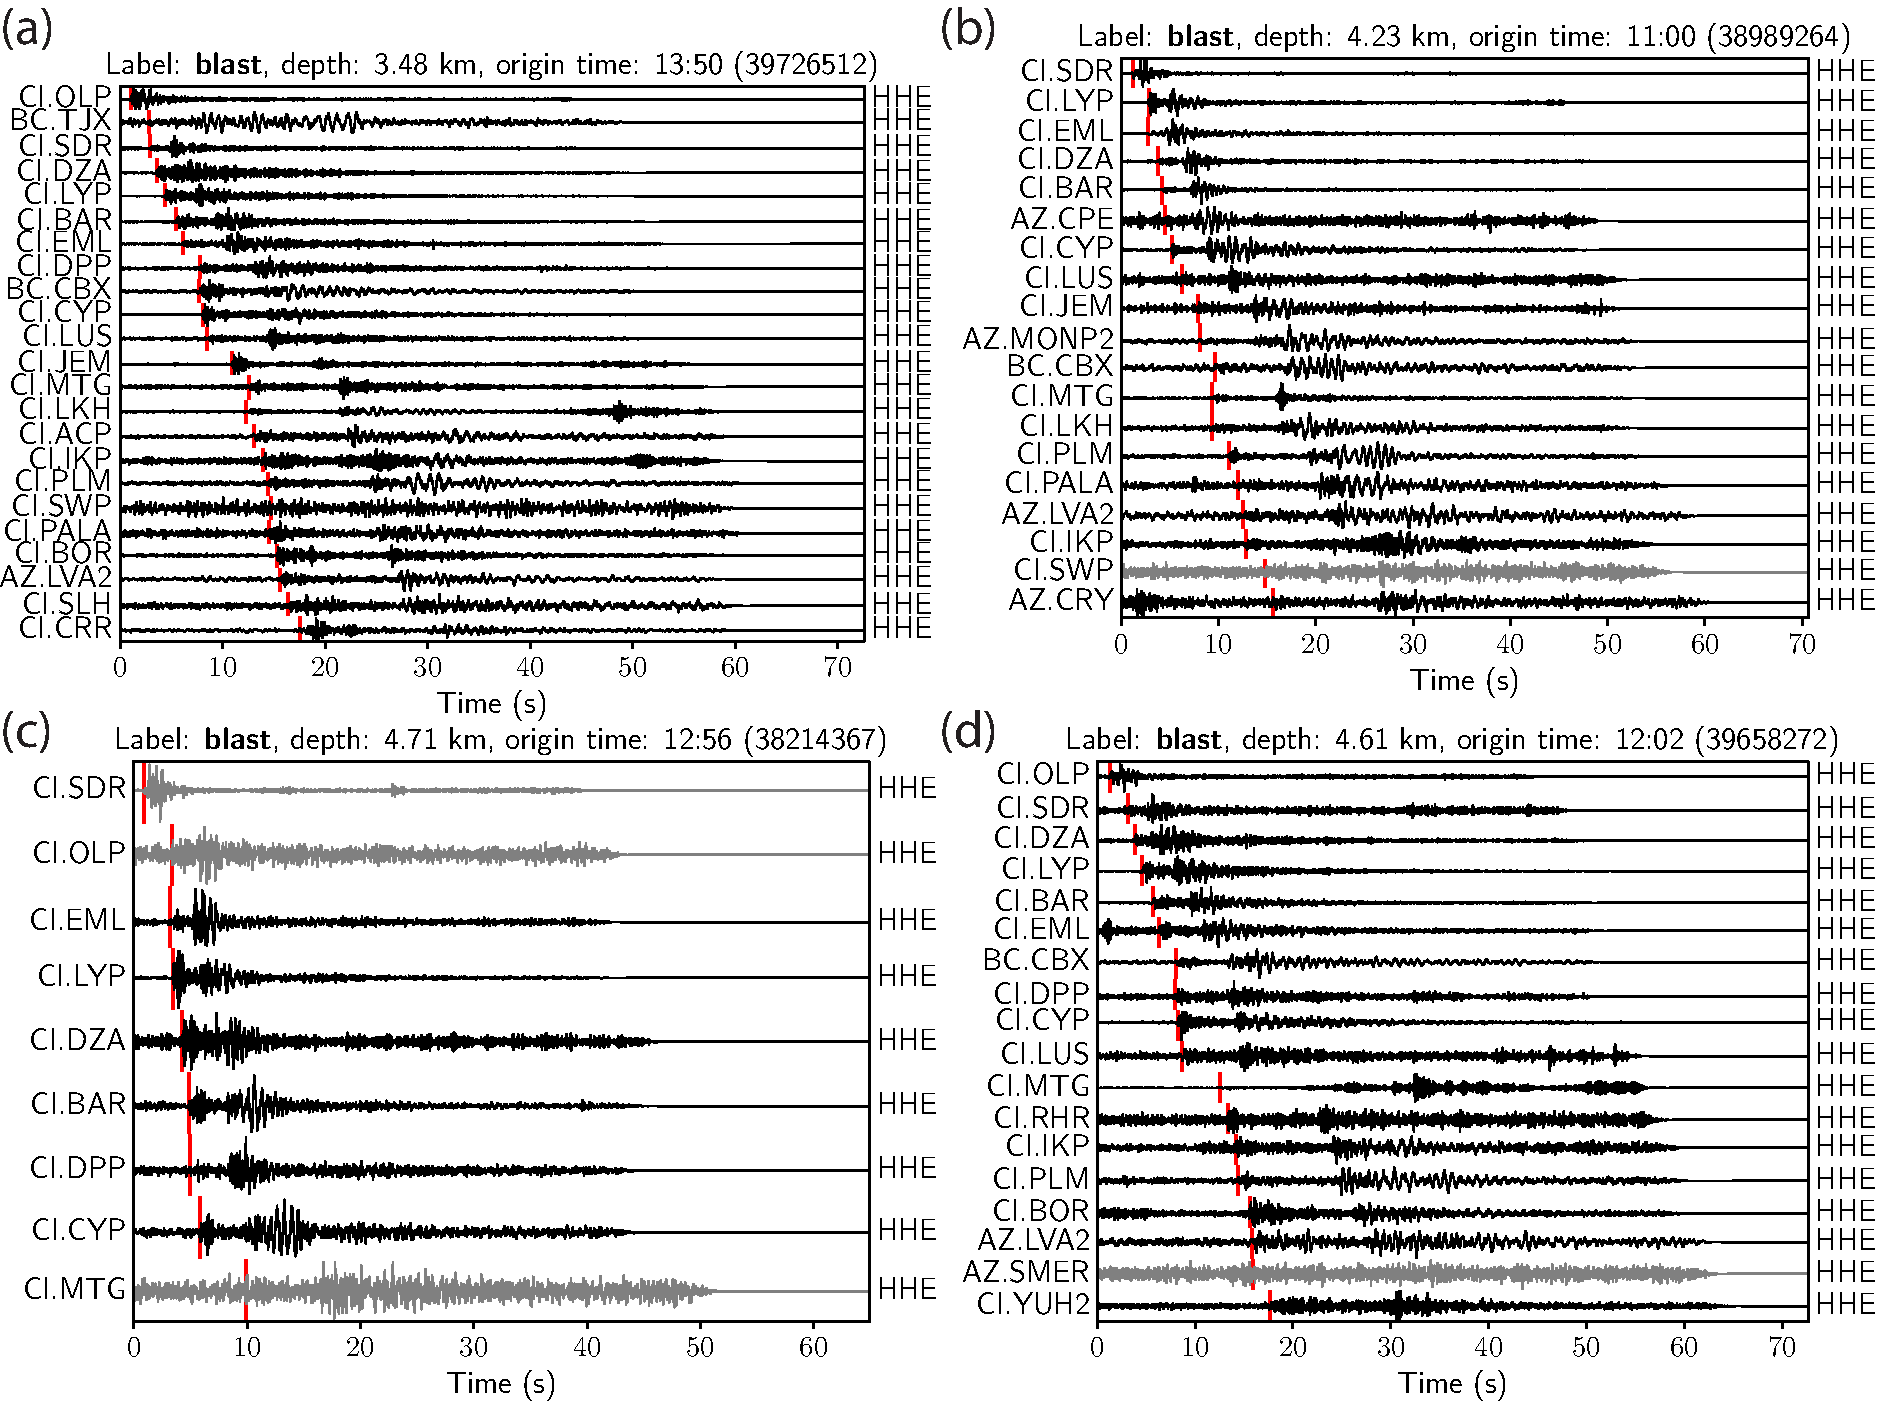
\includegraphics[width=\columnwidth]{deep_blast.pdf}
	\caption{Examples of the anomalously ``deep" events.}
\end{sidewaysfigure}

%\begin{figure}
%	\centering
%	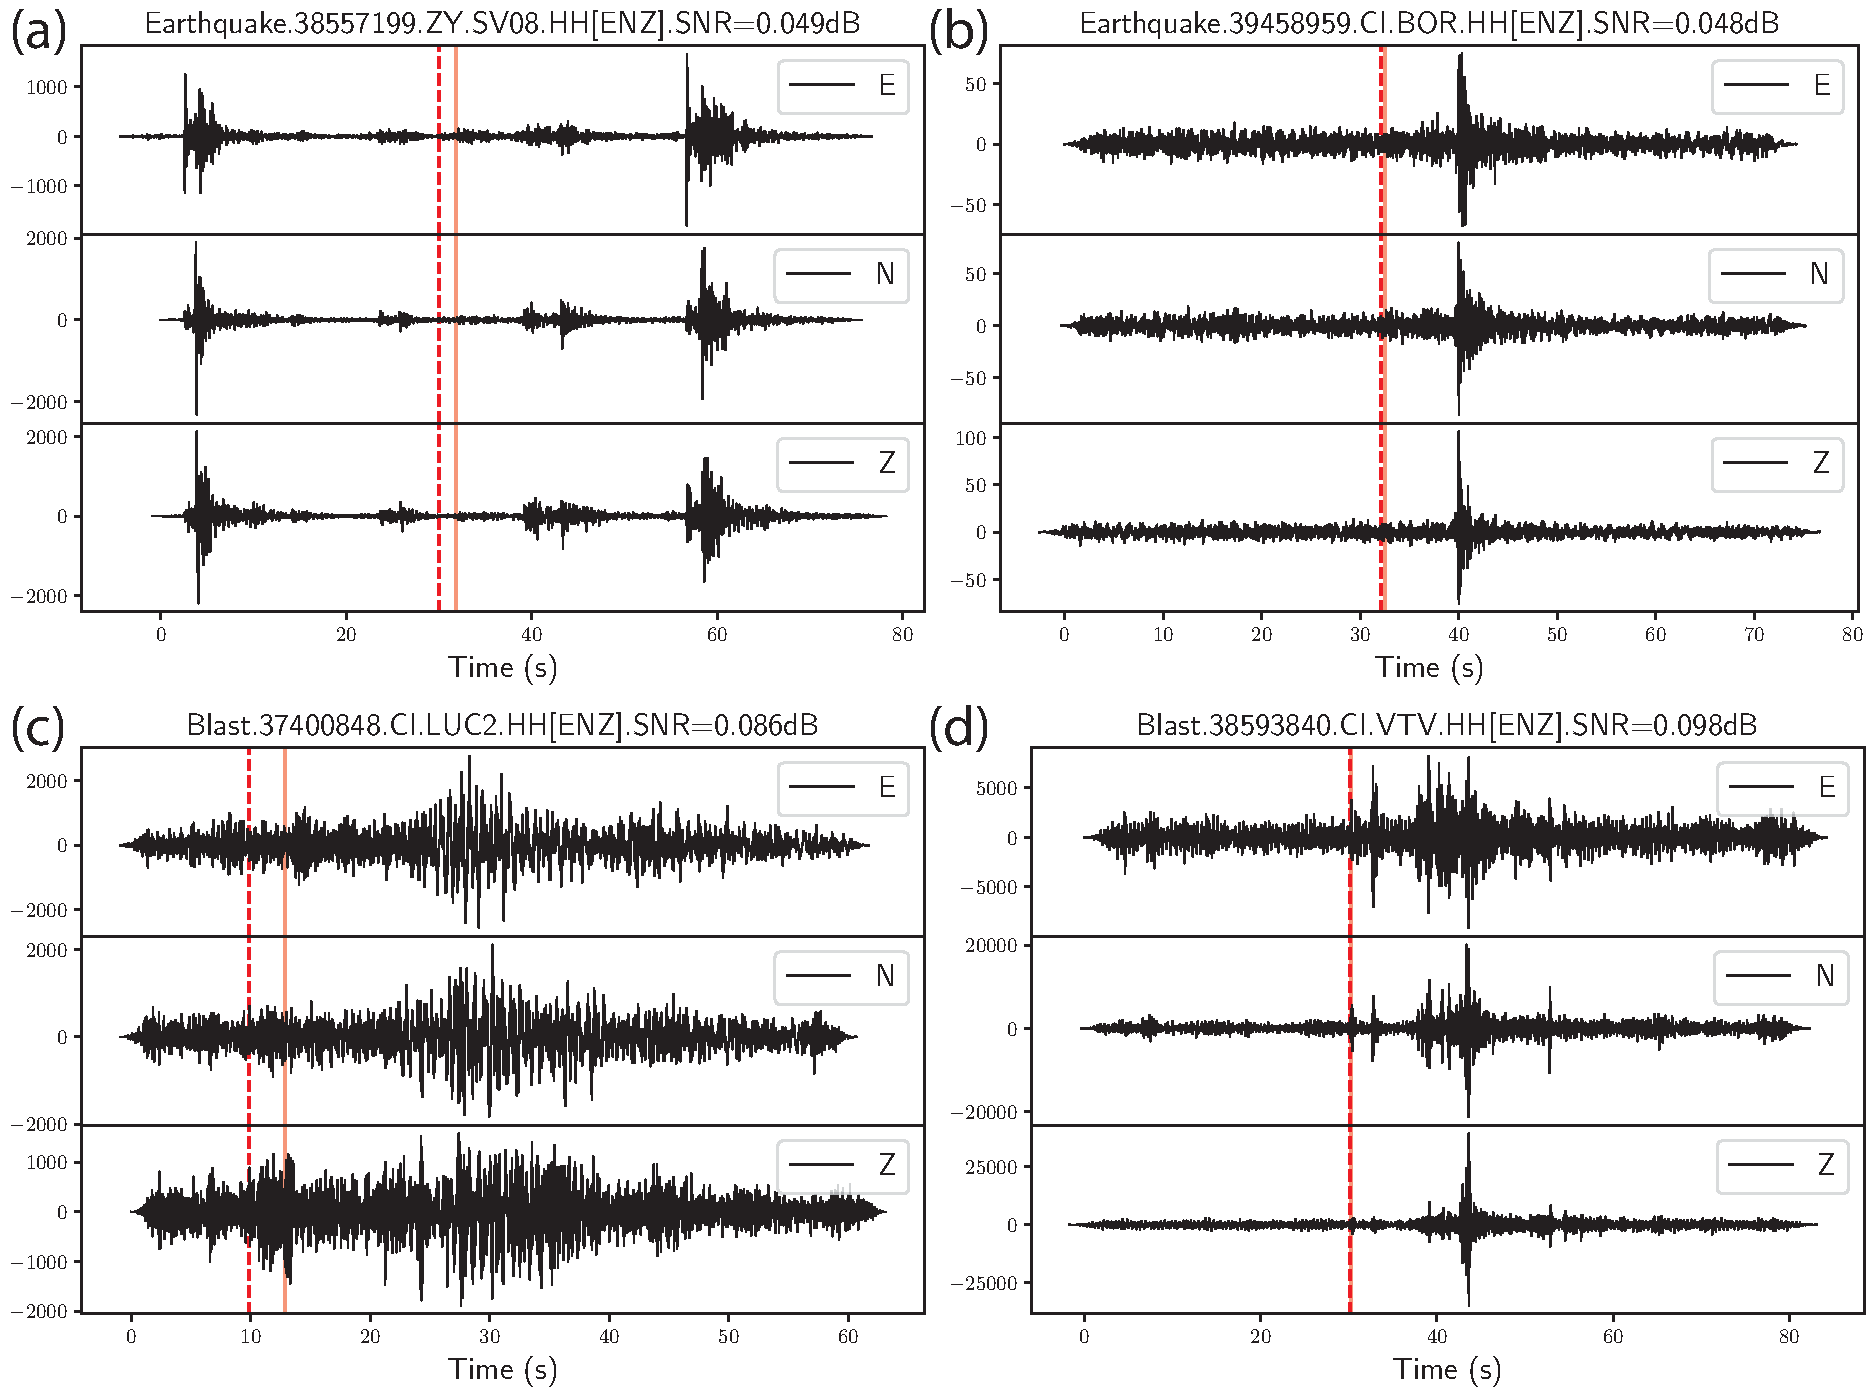
\includegraphics[width=.98\textwidth]{low_snr.pdf}
%	\caption{Low-SNR waveform examples in the California data set.}
%        \label{low_snr}
%\end{figure}

\begin{table}
  \centering
  \begin{threeparttable}[b]
  \caption{Hyperparameters for model training}
    \begin{tabular}{lc}
    \toprule
    Hyperparameter & Value \\
    \midrule
    Initial learning rate & 0.01$^a$ or 0.001$^b$ \\
    Batch size & 128 \\
    Number of convolutional layers & 6 \\
    Dropout rate in the dropout layer & 0.3 \\
    \bottomrule
    \end{tabular}
  \label{hyperparams}
     \begin{tablenotes}
     \item[$a$] An initial learning rate of 0.01 for both the California model and the Kentucky model that are trained from scratch. The initial learning rate will automatically half itself when the validation loss does not decrease for four epochs;
     \item[$b$] For the transferred Kentucky models.
   \end{tablenotes}
\end{threeparttable}
\end{table}

\begin{table}
  \centering
  \begin{threeparttable}[b]
  \caption{Potential mislabels in the California test set}
    \begin{tabular}{ccccccc}
    \toprule
          & Event ID & Event type & Cluster type$^a$ & Origin time & EQ Prob. & Depth (km) \\
    \midrule
    \multirow{7}[2]{*}{False positive} & 39320471 & EQ    & \textbf{QB} & 8:30  & 0.12  & 1.28 \\
          & 38613378 & EQ    & \textbf{QB} & 11:20 & 0.06  & -0.41 \\
          & 38473410 & EQ    & \textbf{QB} & 10:06 & 0.12  & -0.59 \\
          & 39482064 & EQ    & \textbf{QB} & 10:28 & 0.11  & 4.02 \\
          & 39225591 & EQ    & \textbf{QB} & 9:09  & 0.19  & 2.84 \\
          & 39124863 & EQ    & \textbf{QB} & 11:01 & 0.08  & 1.5 \\
          & 39069191 & EQ    & \textbf{QB} & 12:27 & 0.22  & -0.54 \\
    \midrule
    \multirow{9}[2]{*}{False negative} & 38333207 & QB    & \textbf{EQ} & 12:51 & 0.94  & -1.19 \\
          & 39365407 & QB    & QB    & 10:34 & 0.92  & -0.82 \\
          & 39011184 & QB    & QB    & 7:08  & 0.86  & -0.82 \\
          & 39363607 & QB    & \textbf{MIX} & 10:34 & 0.95  & 9.14 \\
          & 39268615 & QB    & \textbf{MIX} & 13:56 & 0.94  & 8.21 \\
          & 39498423 & QB    & \textbf{MIX} & 16:03 & 0.94  & 3.81 \\
          & 39409056 & QB    & \textbf{MIX} & 13:15 & 0.75  & -0.8 \\
          & 37214796 & QB    & \textbf{ISO} & 9:17  & 1     & -0.9 \\
          & 38602752 & QB    & \textbf{ISO} & 12:42 & 0.75  & -0.15 \\
    \bottomrule
    \end{tabular}%
  \label{mislabel}
    \begin{tablenotes}
        \item[$a$] We assign a cluster type to each event as spatial clustering plays a major role in re-evaluating the misclassified events. EQ, cluster of earthquakes. QB, cluster of quarry blasts. MIX, cluster including both types of events. ISO, isolated events without cluster nearby.
    \end{tablenotes}
    \end{threeparttable}
\end{table}%
\end{document}